

\begin{figure}[H]
	\begin{center}
		\begin{minipage}[]{0.49\columnwidth}
			\centering
			\colorbox{white}{ 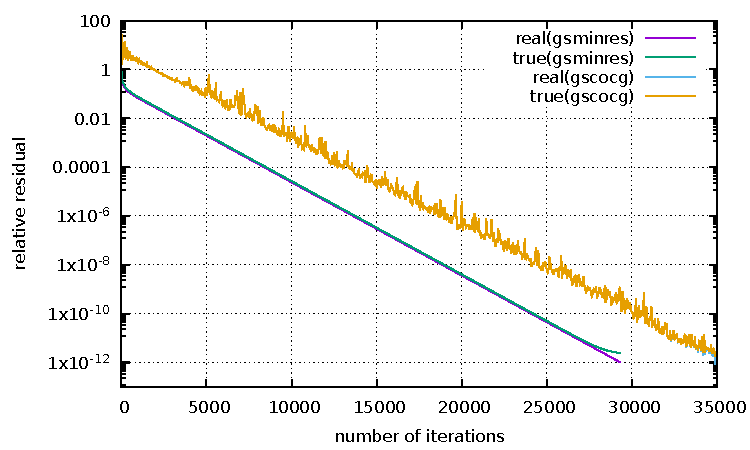
\includegraphics[scale=1.5]{./fig/compare-residual.pdf} }
			\caption{$k=1$における相対残差の比較}
			\label{fig-compare-residual}
		\end{minipage}
		\begin{minipage}[]{0.49\columnwidth}
			\centering
			\makeatletter
			\def\@captype{table}
			\makeatother
			\caption{実行時間と反復回数の比較}
			\label{table-compare-time-itrs}
			\begin{tabular}{ccc}
				\hline
						& 実行時間(秒)	& 反復回数	\\ \hline
				gsminres	& 46			& 3875	\\
				gscocg	& 53			& 4365	\\
				\hline
			\end{tabular}
		\end{minipage}
	\end{center}
\end{figure}

\begin{figure}[H]
	\begin{center}
		\begin{minipage}[t]{0.49\columnwidth}
			\centering
			\colorbox{white}{ 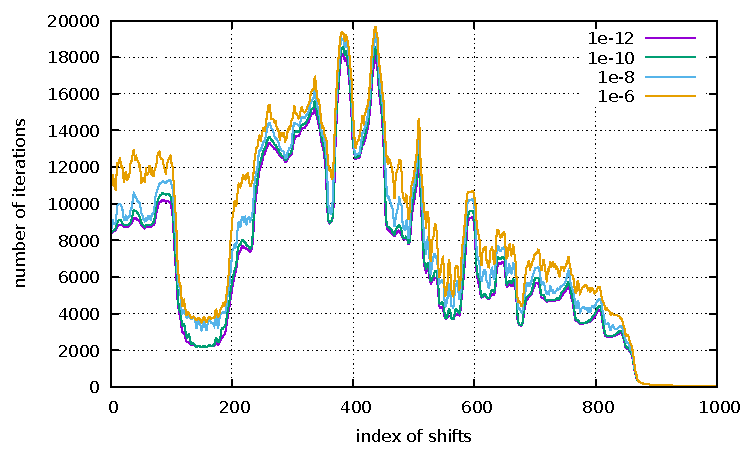
\includegraphics[scale=1.5, page=1]{./fig/compare-inner.pdf} }
			\caption{内部反復の精度と反復回数の比較}
			\label{fig-compare-inner-itr}
		\end{minipage}
		\begin{minipage}[t]{0.49\columnwidth}
			\centering
			\colorbox{white}{ \includegraphics[scale=1.5, page=2]{./fig/compare-inner.pdf} }
			\caption{内部反復の精度の相対残差の関係}
			\label{fig-compare-inner-res}
		\end{minipage}
	\end{center}
\end{figure}

\begin{itemize}
	\item gsminresは滑らかに残差が減少している
		\begin{itemize}
			\item 残差のノルムを最小化しているから
		\end{itemize}
	\item gsminresはアルゴリズム上での残差(real)と真の残差(true)で乖離がある
		\begin{itemize}
			\item $2$--ノルムではなく$B^{-1}$--ノルムの最小化であるから
		\end{itemize}
	\item gsminresがgscocgよりも少ない反復回数で収束し,高速
	\item 外部反復の精度は内部反復の精度程度しかでない
\end{itemize}


\begin{comment}
% https://tex.stackexchange.com/questions/195195/import-pdf-with-white-background


\begin{itemize}
	\item gsminresは滑らかに残差が減少している\\
		\myitem 残差のノルムを最小化しているから
	\item gsminresはアルゴリズム上での残差(real)と真の残差(true)で乖離がある\\
		\myitem $2$--ノルムではなく$B^{-1}$--ノルムの最小化であるから
	\item gsminresがgscocgよりも少ない反復回数で収束し,高速
	\item 外部反復の精度は内部反復の精度程度しかでない
\end{itemize}

\textcolor{structure.fg}{\textbullet} gsminresは滑らかに残差が減少している\\
		\myitem $2$--ノルムではなく$B^{-1}$--ノルムの最小化であるから\\
\textcolor{structure.fg}{\textbullet} gsminresはアルゴリズム上での残差(real)と真の残差(true)で乖離がある\\
		\myitem $2$--ノルムではなく$B^{-1}$--ノルムの最小化であるから\\
\textcolor{structure.fg}{\textbullet} gsminresがgscocgよりも少ない反復回数で収束し,高速\\
\textcolor{structure.fg}{\textbullet} 外部反復の精度は内部反復の精度程度しかでない

\end{comment}